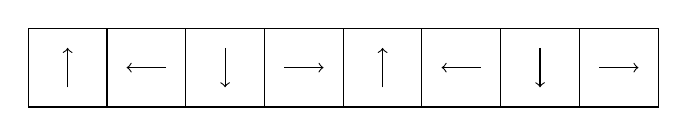
\begin{tikzpicture}
    \foreach \i in {0,...,3}
    {
        \coordinate(1\i) at (0+2*\i,0);
        \coordinate(2\i) at (1+2*\i,0);
        \coordinate(3\i) at (1+2*\i,1);
        \coordinate(4\i) at (0+2*\i,1);
        \draw (1\i) -- (2\i) -- (3\i) -- (4\i) -- cycle;
        \coordinate(5\i) at (1+2*\i,0);
        \coordinate(6\i) at (2+2*\i,0);
        \coordinate(7\i) at (2+2*\i,1);
        \coordinate(8\i) at (1+2*\i,1);
        \draw (5\i) -- (6\i) -- (7\i) -- (8\i) -- cycle;
    }
    
    \foreach \i in {0,...,1}
    {
        \draw[->] (0.5+4*\i,0.25) -- (0.5+4*\i,0.75);
        \draw[->] (1.75+4*\i,0.5) -- (1.25+4*\i,0.5);
        \draw[->] (2.5+4*\i,0.75) -- (2.5+4*\i,0.25);
        \draw[->] (3.25+4*\i,0.5) -- (3.75+4*\i,0.5);
    }

	
\end{tikzpicture}